\documentclass{article}
\usepackage[utf8]{inputenc}
\usepackage{graphicx}
\usepackage[a4paper, total={6in, 9in}]{geometry}
\usepackage{amsmath}
\usepackage{steinmetz}

 
\title{ELEC344 Assignment 1}
\author{Name: Brendan Lai, Student Number: 19241173}
\date{Due: February 15, 2021}
  
\begin{document}
  
\maketitle
  
\tableofcontents

\section{Question 1}
\begin{figure}[h]
    \centering
    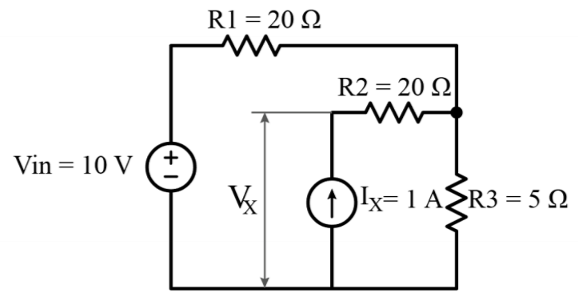
\includegraphics[width=0.6\textwidth]{q1-circuit}
    \label{fig1: q1 circuit}
\end{figure}
Use this circuit to solve the parts of question 1:
    
\section*{Part a:}
Solve the circuit and find the voltage $V_X$. \\
Using KVL over the following two loops we get the two equations:
\begin{align*}
    V_{in} - i_1R_1 - R_3(i_1 - i_x) = 0 \\
    V_x - R_2i_x - R_3(i_1-i_x) = 0
\end{align*}
Substituting and solving the for $i_1$ in $(1)$ we get $i_1 = 0.2$ and consequently use it to solve $(2)$:

\begin{center}
$10 - 20i_1 - 5i_1 - 5(1) = 0$ \\
$V_x - (20)(1) - 5(0.2) - 5(1) = 0$
\end{center}
Solving the second equation we arrive that $V_x = 26 V$

\section*{Part b:}
Add a capacitor of 100 $\mu F$ in parallel with $R_3$ and find the equivalent RC circuit (Thevinin). Calculate the voltage at node A ($V_A = V_{TH}$). Use KCL:\\

\begin{align*}
i_1 + i_2 - i_3 = \frac{V_{in} - V_{TH}}{R_1} + i_x - \frac{V_{TH}}{R_3} = 0
\end{align*}
Rearranging this equation we get that:
\begin{align*}
V_{TH} = (\frac{1}{R_3}+\frac{1}{R_1})^{-1}*(\frac{V_{in}}{R_1} + i_x) = (1/20 + 1/5)^{-1} * (10/20 + 1) 
\end{align*}
Therefore, $V_{TH} = 6V$

Now solving for $R_{TH}$ we set the current source as open and short our voltage source. As a result we get that the resistance seen by the load is $R_1 || R_2$.
\begin{align*}
R_{TH} & = R_1 || R_2 \\
 &= \frac{R_1 R_2}{R_1 + R_2} \\ 
 &= \frac{20*5}{20+5} \\
R_{TH} &= 4 \Omega
\end{align*}

Our Thevinin circuit has the attributes: $R_{TH}=4 \Omega $ and $V_{TH}=6V$

\section*{Part c:}
Find the expression for the capacitor voltage and calculate the time constant for the charging capacitor. \\

Apply boundary conditions assuming that: for $t=0^+ \rightarrow V_c=0$ and for $t=\infty \rightarrow V_C=6V$

\begin{align*} 
    V_s &= V_R(t) + V_c(t) \\ 
    V_c(t) &= V_s(t) - V_R(t) \\
    V_c(t) &= V_s - i_R(t)R 
\end{align*}
We now calculate $i_R(t) = i_c(t) = C \frac{dV_c(t)}{dt}$ 
\begin{align*}
    i_c(t) & = C \frac{d}{dt} (V_s -i(t)R) \\
     & = C(0- \frac{di}{dt}R) \\
     & = - RC \frac{di}{dt} \\
\end{align*}
integrating we get: $i_c(t) = A*e^{-t/RC} = \frac{V}{R} e^{-t/RC}$

Let $RC = \tau$  a time constant then $\tau = 4 * 100*10^{-6} = 0.4$  milliseconds

\section*{Part d:}
The PSIM circuit I used and the relevant waveform during the capacitor charging transient was:
\begin{figure}[h]
    \centering
    \includegraphics[width=0.6\textwidth]{Psim-Q1-circuit}
    \includegraphics[width=0.9\textwidth]{psim-q1-Graph}
    \label{PSIM circuit q1}https://www.overleaf.com/project/602607a08bfffe516682ded1
\end{figure}


\section{Question 2}
Using the following circuit with an input power supply $V_{in}=\sqrt{2}*110 \sin{(\omega t)}$ and $f=60Hz$
\begin{figure}[h]
    \centering
    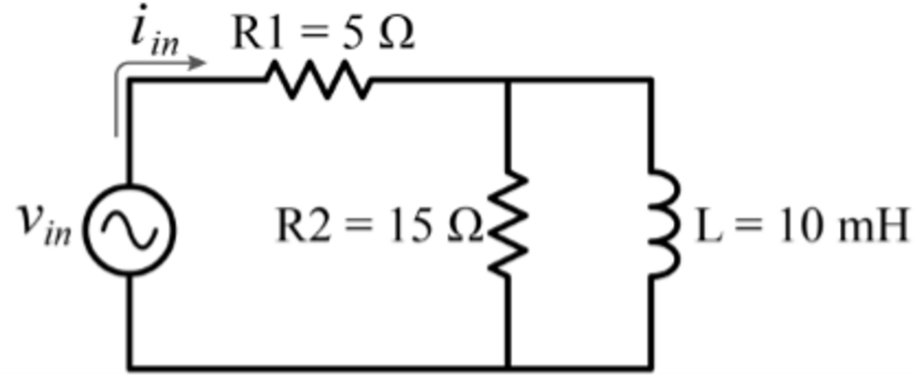
\includegraphics[width=0.5\textwidth]{q2-circuit}
    \label{q2 circuit}
\end{figure}
\section*{Part a:}
Calculate magnitude and phase of the input current.

Calculate the circuits equivalent impedance $Z_{eq}$:
\begin{align*}
    Z_{eq} & = Z_{R1} + Z_{RL} = Z_{R1} + (Z_{R2} || Z_{L}) = R_1 + (R_2 || (j \omega L)) \\
    Z_{eq} & = 5 + ( 15 || (j (120 \pi)(10 * 10^{-3})) ) \\
    Z_{eq} & = 5.89119 + j 3.54594
\end{align*}

Note: To calculate between polar and rectangular form: 
\begin{center}
    $Magnitude = \sqrt{(real)^2 + (imaginary)^2}$ and $Phase = \arctan{\frac{imaginary}{real}}$
\end{center}

Then calculate the input current using $i_{in} = V_{in} / Z_{eq}$:

\begin{align*}
    i_{in} &= \frac{\sqrt{2}*110*\sin{(120\pi t)}}{5.89119 + j 3.54594} = \frac{\sqrt{2}*100 \phase{0^{\circ}} }{6.87603 \phase{31.0469^{\circ}}}\\
    i_{in} & = 20.5673  \phase{-31.0439^{\circ}} 
\end{align*}

As we can see the input currents magnitude and phase are: $20.6A$ and ${-31.0^{\circ}}$ respectively

\section*{Part b:}
Adding a capacitor in parallel with the inductor, calculate the value of the capacitor to obtain 0 degree phase shift between the input current and voltage \\

To have a zero phase shift between our current and voltage they must be in phase. This means that our capacitance load must incur a phase shift equal but opposite to the phase imposed by our inductor. $Z_L + Z_C = 0$

Our $Z_L$ phase is:
\begin{align*}
    Z_L &= -Z_C \rightarrow
    j(\omega L) = \frac{-1}{j (\omega C)}  \rightarrow
    \omega L =\omega C
\end{align*}
Now solve for the capacitance C:
\begin{align*}
    C &= \frac{1}{\omega^2 * L} =\frac{1}{(120 \pi)^2(10*10^{-3})}\\
    C &= 7.03619 * 10 ^{-4}
\end{align*}
Therefore to achieve zero phase shift between our input voltage and current you would need to add a $703.6 \mu F$ capacitor in parallel to the inductor.

\section{Question 3}
Use the shown ideal 3-phase rectifier with the following parameters to solve each part

\begin{center}
\begin{tabular}{ c   c }
    $v_a = \sqrt{2} * 120\sin{(\omega t)}$ & $\omega = 2 \pi f$ \\ 
    $v_b = \sqrt{2} * 120\sin{(\omega t +120^{\circ})}$ & $f=60Hz$  \\  
    $v_c = \sqrt{2} * 120\sin{(\omega t -120^{\circ})}$ & $R = 10 \Omega$   
\end{tabular}
\end{center}

\begin{figure}[h]
    \centering
    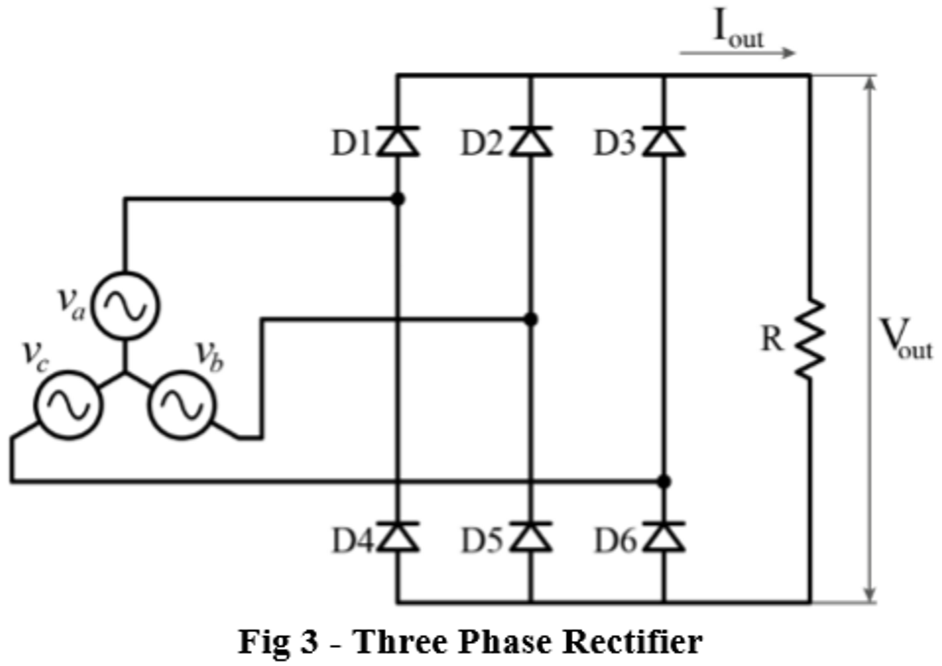
\includegraphics[width=0.45\textwidth]{q3-circuit}
    \label{Circuit q3}
\end{figure}

\section*{Part a:}
Calculate the amplitude of the output voltage and current. \\

The output voltage will be equivalent to the line to line voltage of the 3 phase voltage. Using the derivation from tutorial we know that $V_{L-L} = \frac{V_{phase)}}{\sqrt{3}}$. We also know that $I_{out} = V_{out} / R$. Therefore:
\begin{align*}
    V_{out} = \sqrt{3}*\sqrt{2}*120 = 293.94 V \\
    I_{out} = \frac{V_{out}}{10} = 29.39 A
\end{align*}

\section*{Part b:}
Simulate the circuit in Fig. 2 using PSIM and plot the output voltage, output current and current in each diode. 
\begin{figure}[h]
    \centering
    \includegraphics[width=0.75\textwidth]{Psim-Q3}
    \label{PSIM circuit q3}
\end{figure}
\begin{figure}[h]
    \centering
    \includegraphics[width=0.9\textwidth]{psim-q3-Graph}
    \label{PSIM circuit q3}
\end{figure}

\section*{Part c:}
Explain the observations from the waveforms. What diodes are conducting at each portion of time? What is the conduction angle for the diodes and explain. \\ \\
From the plots one observation to make is that pairs of diodes are on at the same time. The pairs of being on are in sequence and are (D1-5, D1-6, D2-6, D2-4, D3-4, D3-5). Each pair of diodes are on for a $\frac{\pi}{3}$ or $60^{\circ} $ time step $\rightarrow t=\frac{60}{2\pi60 }= 0.1592 s$ while each individual diode is on for $\frac{2 \pi}{3}$ or $120^{\circ} $ time step $\rightarrow t = 0.3183s $. \\
The active diodes are dependent on the phase voltage that is most positive and most negative at that time. Also given our frequency (60Hz) and phase shift ($120^{\circ}$) the change between each voltage wave is continuous and activites different diodes each time in a cycle

\section{Question 4}
The circuit below is used to control the brightness of LEDs by using PWM modulating with a digital microcontroller. LEDs work as rectifier diodes and its brightness is proportional to the average current that passes through the diode $(i_d)$.
\begin{figure}[h]
    \centering
    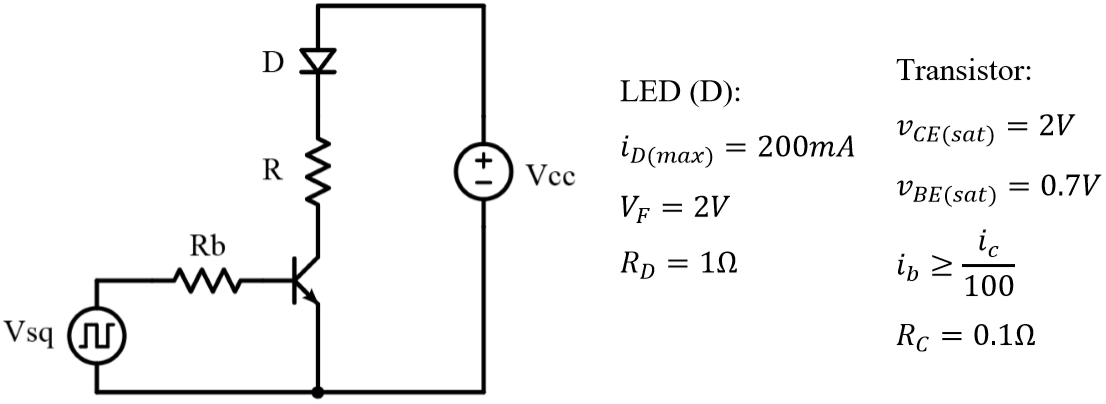
\includegraphics[width=0.85\textwidth]{q4-circuit}
    \label{q4 circuit}
\end{figure}

\section*{Part A:}
For $V_{CC} = 5V$ calculate:
\begin{itemize}
    \item Value of resistor R necessary for full brightness when the transistor is continuously ON
    \item Maximum value of the resistor $R_b$ that enables such condition
    \item Average diode power $(P_D)$, resistor power $(P_R)$, transistor power $(P_T)$, and source power $(P_{VCC})$ for 50\% brightness
\end{itemize}

To calculate the resistor for full brightness assume the maximum current for $i_D$ and $V_{CE}$ is saturated. As a result we can perform KVL on the right sided loop.

\begin{align*}
    V_{CC} - V_F - (i_D*R_D) - (i_D * R) - V_{CE} = 0
\end{align*}

Substitute the values in and solving for R we get:
\begin{align}
    R = 5 (5-2-(0.2*1)-2) = 4\Omega
\end{align}
\\ To calculate the maximum value of $R_B$ we can perform KVL on the left sided loop taking the minimum current $i_B = 200mA / 100 = 2mA$
\begin{align*}
    V_{sq} - V_{BE} - (i_b * R_B) = 0
\end{align*}
Substitute the values in and solving for $R_b$ we get:
\begin{align}
    R_b = (5 - 0.7)*(2*10^{-3})^{-1} = 2.15 k\Omega
\end{align}

Assuming that 50 \% brightness is when $V_{sq}$ is on 50 \% of the time then the transistor power can be calculated using $V_{CE} * i_C$. We can also calculate the resistor power individually and identify the source power using the source voltage and current in the wire. As a result, each 

\begin{align*}
    P_T &= v_{CE} *i_C * (1/2) =2V * 200 mA *(1/2) = 0.2 W \\
    P_R &= R*i_d^2 * (1/2) = 4 * 0.2^2 * (1/2) = 0.08 W \\
    P_{V_{CC}} &= V_{CC} * i_D * (1/2) = 5 * 0.2 * (1/2) = 0.5W \\
\end{align*}
Using these values we can finally calculate the power from the diode using the conservation of power. $\Sigma (P) = 0$
\begin{align}        
    P_D = P_{V_{C}} - P_R - P_T = 0.5 - 0.08 - 0.2 = 0.22W
\end{align}

\section*{Part B:}
Repeat the calculations performed in (part A) but for $V_{CC} = 12V$

Use the same approach as on part a of this question
\begin{align*}
    V_{CC} - V_F - (i_D*R_D) - (i_D * R) - V_{CE} = 0
\end{align*}

Substitute the values in and solving for R we get:
\begin{align}
    R = 5 (12-2-(0.2*1)-2) = 39\Omega
\end{align}

The maximum value of $R_b$ remains unchanged from part A.
\begin{align}
    R_b = (5 - 0.7)*(2*10^{-3})^{-1} = 2.15 k\Omega
\end{align}

Use the same approach of manipulating the conservation of power to calculate $P_D$.

\begin{align*}
    P_T &= v_{CE} *i_C * (1/2) =2V * 200 mA *(1/2) = 0.2 W \\
    P_R &= R*i_d^2 * (1/2) = 39* 0.2^2 * (1/2) = 0.78 W \\
    P_{V_{CC}} &= V_{CC} * i_D * (1/2) = 12 * 0.2 * (1/2) = 1.39
\end{align*}
\begin{align}        
    P_D = P_{V_{C}} - P_R - P_T = 0.5 - 0.08 - 0.2 = 0.22W
\end{align}
As a result we can conclude that the power of the diode doesn't change. This is that when $V_{CC}$ changed the power of the diode remains the same.

\end{document}